\documentclass[a4paper,10pt,twocolumn]{article}
\usepackage{lmodern}
\usepackage[czech]{babel}
\usepackage[T1]{fontenc}
\usepackage[utf8]{inputenc}
\usepackage{graphicx}
\usepackage{float}
\usepackage{amsmath}
\usepackage{amssymb}
\usepackage{svg}
\usepackage[top=0.5cm,bottom=2cm,left=1cm,right=1cm]{geometry}

\pagenumbering{gobble} 
\title{Zpráva k semestrální práci z předmětu BI-ZUM}
\date{\today}

\author{Ladislav Macoun\\ macouladl@fit.cvut.cz}

\newcommand\tab[1][1cm]{\hspace*{#1}}

\begin{document}
\maketitle
\begin{abstract}
V této práci jsem se zabýval vylepšením genetického algoritmu (GA) pro optimalizační problém minimalního hránového pokrytí v grafu. GA jsem vylepšil o adaptivní přizpůsobení volby pravděpodobnosti křížení a mutace \cite{adga}, dálé regenerací populace při katastrofální konvergenci fitness a deterministické shlukování\cite{dc}\cite{ga} (Deterministic crowding). Dále je vylepšená inicializace podle heuristiky hledání optimálního řešení pokrytí vrcholů s vetší váhou.
\end{abstract}

\section{Parametry algoritmu}
Genom je reprezentován binární kombinací True (vrchol je označen) a False (vrchol není označen),
kde na začátku běhu GA se vytvoří gen odřezaných listů. Tento gen jak pak maskou při vytváření nových genomů a optimalizuje volbu náhodně volených genomů.
Fitness funkce $f(X_i)$ jedince $X_i$ je dána vztahem 
$$f(X_i)=\exp(\log \sum_{n=1}^{n}
\begin{cases}
X_i[k] == 1, -1\\
X_i[k] == 0, +1\\
\end{cases})$$
kde $X_i[k]$ je hodnota genomu na k-tém místě jedince $X_i$, a n je délka genomu jedince $X_i$.
Velikost populace jsem zvolili $65$, počet generací $2500$ a nejvyšší pravděpodobnost mutace $\pi_{max}$ = $0,03$, $\pi_{min}$ = $0,035$ a pravděpodobnost křížení $\pi_{max}$ = $0,75$ a $\pi_{min}$ = $0,3$. 

\section{Operátor mutace}
Při mutaci chceme, aby v počátečních generacích vývoje byla pravděpodobnost mutace vyšší a vylepšila diverzitu. Proto je zvolena adaptivní pravděpodobnost mutace \cite{adga} $\pi_{\mu}$, která je dána vztahem 
$$\pi_{\mu} = \exp(\frac{f_{max} - f(X_i)}{f_{max}}) \cdot \frac{\pi_{max} - \pi_{min}}{\frac{1 + \exp(-\alpha(\tau_{Gen} - 2\tau))}{\tau_{Gen}}}) + \pi_{min} $$
kde $f_{max}$ je maximální hodnotna fitness funkce, $f(X_i)$ je fitness hodnota jedince $X_i$, dolní $\pi_{min}$ a horní $ \pi_{max}$ omezení pravděpodobnosti mutace. Tímto docílíme toho, že pravděpodobnost $\pi_{\mu}$ se bude měnit v závislosti na fitness daného jedince a konkrétní generaci.

\section{Operátor křížení}
Jako operátor křížení je použito jednobodové křížení s pevným bodem řezu uprostřed genomu.
Adaptivní pravděpodobnost křížení \cite{adga} je volená v závislosti na vývoji generací a je dána vztahem
$$\pi _\gamma (t) = \frac{\pi_{min} - \pi _{max}}{1 + exp(\frac{-\alpha \tau_{gen} - 2 \tau }{\tau_{gen}})} + \pi_{min}$$
kde $\pi_{min}$ je minimální pravděpodobnost, $\pi_{max}$ je maximální pravděpodobnost, $\tau$ je
současná generace, $\tau_{gen}$ je počet generací a řídící operátor $\alpha$ je zvolen na $9,903438$\cite{adga}.
Tímto vztahem získáme vetší pravděpodobnost křížení v počátečních generacích, které se postupně snižuje.

\section{Selekce}
Pro selekci je využíván turnaj, při kterém se náhodně vybere $5$ jedinců, ze kterých se vybere ten s nejvyšší fitness hodnotou.\\
Pseudokódem :\\
$
SelectIndividuals( amount ) :\\
	\tab \Sigma = \emptyset, \Theta_{random} = \emptyset\\
	\tab while |\Sigma| \  != amount \ do:\\		
		\tab \tab while |\Theta_{random}| \  != \  5\\
			\tab \tab \tab \Theta_{random} = \ \Theta_{random} \cup X_{random}\\
			\tab \tab \tab \Sigma = \Sigma \ \cup fittest \in \Theta_{random}\\
	\tab return \  \Sigma\\
$
Díky náhodnému zvolení jedinců v turnaji zajistíme diversitu v genomu.

\section{Vývoj hodnoty fitness}
\begin{figure}[H]
   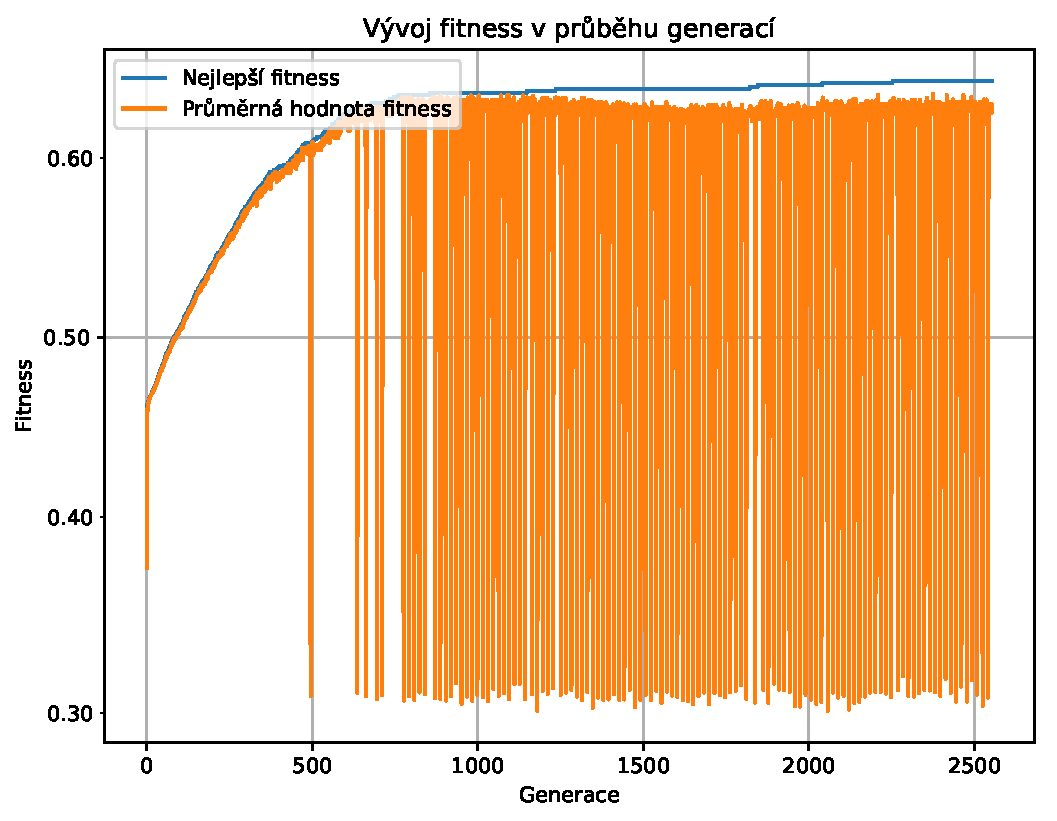
\includegraphics[width=9cm,height=3cm]{graph.pdf}
  \caption{Graf vývoje fitness}\label{fig1}
\end{figure}
V grafu je vidět, že ke konci GA konverguje k lokálnímu maximu, a spouštějí se čím dál časteji katastrofické regenerace populace. Toto je pravděpodobně způsobené elitismem při výběru nových jedinců.

\section{Shrnutí a výsledky}
GA dokáže najít řešení blizké optimálnímu v poměrně krátké době při zvolené nízké populaci. Zlepšení nejlepší fitness z první generece, která činí $0.35$ na $0.64$, je zlepšení o $178.08\%$ a to v čase $48218$ ms. Toto by se dalo urychlit generováním nových jedinců pomocí vícevláknového zpracování. Je možné že by se dalo dosánout lepších výsledků s jinými parametry pro GA, jako jsou omezení pravděpodobností mutací, kříženi a velikost populace. Dále by se dala zoptimalizovat regenerační funkce populace o adaptivní operátor výběru počtu přeživších \cite{adga}. 

\bibliographystyle{iso690}
\bibliography{citations}

\end{document}
